
\section{Video Analysis Using Tracker}

\textbf{Making a Movie with ``Movie Maker''} 

To make a movie, perform the following steps:

\begin{enumerate}

\item Make sure the camera is connected to a USB port on your computer. 
Close all windows, applications, programs, and browsers.

\item Click the {\bf Start} button in the lower-left corner of your screen and 
type `movie maker' in the Search programs and files box. 
Once the search results appear, click on {\bf Movie Maker} at top of window.
After movie maker starts, close any pop-up windows that may appear.

\item Click the {\bf Webcam Video} button. 
A webcam video window opens. 
%Enlarge the video frame by dragging the vertical line on the right side of the video frame.

\item Position the camera 2-3 meters from the object you will be viewing. 
Adjust the camera height and orientation so that the field of view is 
centered on the expected region where the object will move. 

\item Place a meter stick or an object of known size in the field of view where 
it won't interfere with the experiment. 
The meter stick should be the same distance away from the camera as the motion 
you are analyzing so the horizontal and vertical scales will be accurately determined. 
It should also be parallel to one of the sides of the movie frame. 
Make sure that the meter stick is not far away from the central region of field of view, and that it is perpendicular to the line of sight of camera.

\item One member of your group should perform the computer tasks while the other does the experiment.

\item To start recording your video, click {\bf Record}. When you are done, click {\bf Stop}. 

Save the video on your Desktop with a unique name that you can easily identify.
 The video will be saved in Windows Media Video format, i.e. with extension wmv. (Do not save the video as a Movie Maker Project file.)

\end{enumerate}

\textbf{Analyzing the Movie} 

To determine the position of an object at different times during the
motion, perform the following steps:

\begin{enumerate}

\item Start up Tracker by going to {\bf Start} $\rightarrow$ {\bf Programs} $\rightarrow$ {\bf Physics Applications} $\rightarrow$ {\bf Tracker}. 
When {\bf Tracker} starts it appears as shown below. The menu icons and buttons that we will use are identified by arrows.
\begin{figure}[hbt]
\begin{center}
\includegraphics[width=5.5in]{Tracker_figure.eps}
\caption{Initial {\bf Tracker} window for video analysis.}
\end{center}
\end{figure}

\item Click the {\bf Open Video} button on the toolbar to import your video. 
After your video is imported, Tracker will warn you that the video frames 
don't have the same time duration. 
This is okay since Movie Maker uses a variable frame rate. 
Click {\bf OK} on the warning window to ignore Tracker's recommendation.

\item Click the {\bf Clip Settings} button to identify the frames you wish to analyze. 
A clip settings dialog box appears. 
Here, you only need to identify and set the start and end frames. 
Leave everything else in the dialog box unchanged. 
To find and set the start frame, drag the player's left slider to scan forward through the video, and 
stop when you get to the first frame of interest. 
Now, the start frame is set and the corresponding frame number should be displayed in the dialog box. 
If not, then click on the {\bf Start Frame} in the dialog box, enter the number of the frame 
(printed in the lower left part of the Tracker window), and click outside the box.
Then, click the {\bf Play video} button to go to the last frame in the video. 
Next, drag the player's right slider to scan backward through the video to find the last frame of interest. 
Stop when you get to the frame of interest. Now, the end frame is also set and the corresponding frame number should be displayed in the dialog box. 
If not, then click on the {\bf End Frame} in the dialog box, enter the number of the frame, and click outside the box.
Finally, click the {\bf OK} button to close the dialog box, and then click the player's {\bf Return} button to return to the start frame.

\item Click the {\bf Calibration} button and select the {\bf calibration stick}. 
A blue calibration line appears on the video frame. 
Drag the ends of this blue line to the ends of your calibration meter stick. 
Then click the readout box (the number indicating length) on the calibration 
line to select it. 
Enter the length of the meter stick in this box (without units). 
For example, if your calibration meter stick is 1.00 meter long, enter 
1.00 in the box (if not already there) 
and then click outside the box to accept the value. 
At this point, you can right-click the video frame to zoom in for more accurate adjustment of the ends of the calibration stick. 
Right-click the video again to zoom out.

\item Click the {\bf Axes} button to set the origin and orientation of the x-y coordinate axes. 
Drag the origin of the axes to the desired position (in most cases the initial position of the object of interest). 
Click the video outside the origin to fix the position of the origin. 
To change the orientation (angle) of the axes, drag the x axis. 
Click the video to fix the new orientation.

\item Click the {\bf Create} button to track the object of interest in the video. 
From the menu of choices select {\bf Point Mass} for the track type. 
Make sure the video is at the start frame, which shows the initial position of the object of interest. 
Mark this position by holding down the {\bf shift key} and clicking the mouse (crosshair cursor) on the object. 
As the position is marked, the video automatically advances to the next frame. 
Similarly, mark the position of the object on this and subsequent frames by holding down the {\bf shift key} and clicking the mouse. 
Do not skip any frames. 

After marking the position on the end frame, you can adjust any one of the marked positions. 
Advance the video to the frame where you would like to make a fine adjustment. 
Right-click the video frame to zoom in and drag the marked position with the mouse.

If you would like to track additional objects, repeat the procedure outlined here for each object.

\item {\bf Plotting and Analyzing the Tracks:} The track data (position versus time) are listed in the Table View and plotted in Plot View sections of the Tracker screen. Click the vertical axis label of the plot to change the variable plotted along that axis. To plot multiple graphs, click the {\bf Plot} button, located above the plot, and select the desired number. 
Right-click on a plot to access display and analysis options in a pop-up menu. To fit your data to a line, parabola, or other functions, select the {\bf Analyze} option. On the Data-Tool window that opens up, click the {\bf Analyze} button and check the {\bf Curve Fits} box from the drop-down menu. Then select the fit type from the {\bf Fit Name} drop-down menu (lower left). Make sure the {\bf Auto fit} box is checked. 
Note that the curve fitter fits the selected function to the data in the two leftmost columns of the displayed data table. The leftmost column, identified by a yellow header cell, defines the independent variable, and the second leftmost column, identified by a green header cell, defines the dependent variable. So, to fit the data in other columns, their corresponding headers must be dragged to the two leftmost columns. To print out the displayed plot and data table on the Data Tool screen, select {\bf Print} from the {\bf File} menu on the Data Tool screen.

\item {\bf Printing and Exporting Data:} Track data can also be easily exported to Excel for further analysis by copying the data from the data table to the clipboard and pasting into Excel. 
%Click the {\bf Table} button, located above the data table in the table view section of the main screen, and select from the displayed list the data you would like to display in the data table. Select the desired data in the table, then right-click and choose {\bf Copy Data} from the pop-up menu. Now, paste the data into Excel.
%To print out the displayed  plot or data table on Tracker's screen, right-click on the plot or table and choose {\bf Print} from the pop-up menu.
Select the desired data (on Data Tool screen), go to {\bf Edit} $\rightarrow$ {\bf copy} $\rightarrow$ {\bf selected data} (on Data Tool screen). 
Open Excel (in Microsoft Office folder) and click the Paste clipboard. Data should appear in Excel. Graph can now be plotted in Excel (see {\bf Appendix C: Introduction to Excel}) and printed.

\end{enumerate} 

